\documentclass{beamer}

\usepackage{tikz}
\usetikzlibrary{matrix}
\usepackage{fancyvrb}
\usepackage{movie15}

%\usepackage{tieto}
\usetheme{Warsaw}

\title{Inside-Out: STL}
\subtitle{How to use it wisely?}
\author{Jadwiga Pokorska}
\institute{TietoEvry}
\date{26.02.2020}

\tikzset{
  invisible/.style={opacity=0},
  visible on/.style={alt={#1{}{invisible}}},
  alt/.code args={<#1>#2#3}{%
    \alt<#1>{\pgfkeysalso{#2}}{\pgfkeysalso{#3}} % \pgfkeysalso doesn't change the path
  },
}

\begin{document}
    %\usebackgroundtemplate{\includegraphics[width=\paperwidth,height=\paperheight,keepaspectratio]{Tieto_title.jpg}}

\begin{frame}
\titlepage
\end{frame}

\begin{frame}
\frametitle{Presentation plan}
\tableofcontents
\end{frame}

\section{Introduction}

\subsection{Time complexity}
\begin{frame}
    \frametitle{Time complexity}
    \begin{block}{Purpose}
    Time complexity is a tool to measure the efficiency of our algorithm.
    \end{block}

    \pause
    Usually defined with \textit{big-O} notation:
    \begin{itemize}
        \item $O(N)$,
        \item $O(N^2)$,
        \item $O(\log N)$,
        \item $O(N \cdot \log N)$,
        \item $O(\sqrt N)$,
    \end{itemize}
\end{frame}


\begin{frame}
    \frametitle{Task: find not paired item}
    \begin{block}{Task}
        Given an array of integers, find the only number that does \textbf{not}
        have a pair.
    \end{block}

    \pause
    \begin{example}
    For array $[2, 3, 7, 7, 2, 3, 2]$ the answer is $2$.
    \end{example}
\end{frame}

\begin{frame}[fragile]
    \frametitle{Task: find not paired item}
    \begin{verbatim}
int find_not_paired(const vector<int>& t) {
    for (int selected_item : t) {
        int cnt = 0;
        for (int item : t)
            if (item == selected_item)
                cnt++;
        if (cnt % 2 == 1)
            return selected_item;
    }
    return 0;
}\end{verbatim}

    \begin{block}{}
    What is the time complexity? \pause \textcolor{red}{$O(N^2)$}
    \end{block}
\end{frame}

\begin{frame}[fragile]
    \frametitle{Task: find not paired item}
    \small
    \begin{verbatim}
int find_not_paired(const vector<int>& t) {
    sort(t.begin(), t.end());
    int cnt = 0, prev = -1;
    for (int i = 0; i < t.size(); ++i) {
        if (prev == t[i]) cnt++;
        else {
            if (cnt % 2 == 1) return prev;
            prev = t[i];
            cnt = 0;
        }
    }
    if (cnt % 2 == 1) return prev;
    return 0;
}\end{verbatim}

    \begin{block}{}
    What is the time complexity? \pause \textcolor{red}{$O(N \cdot \log N)$}
    \end{block}
\end{frame}

\begin{frame}[fragile]
    \frametitle{Task: find not paired item}
    \begin{verbatim}
int find_not_paired(const vector<int>& t) {
    int result = 0;
    for (int item : t)
        result ^= item;
    if (result > 0)
        return result;
    return 0;
}\end{verbatim}

    \begin{block}{}
    What is the time complexity? \pause \textcolor{red}{$O(N)$}
    \end{block}
\end{frame}

\begin{frame}[fragile]
    \frametitle{Task: find not paired item}
    \begin{verbatim}
int find_not_paired(const vector<int>& t) {
    map<int,int> m;
    for (int item : t)
        m[item]++;
    for (auto it : m) {
        if (it.second % 2 == 1)
            return it.first;
    }
    return 0;
}\end{verbatim}

    \begin{block}{}
    What is the time complexity? \pause \textcolor{red}{$O(N \cdot \log N)$}
    \end{block}
\end{frame}

\begin{frame}[fragile]
    \frametitle{Task: find not paired item}
    \begin{verbatim}
int find_not_paired(const vector<int>& t) {
    unordered_map<int,int> m;
    for (int item : t)
        m[item]++;
    for (auto it : m) {
        if (it.second % 2 == 1)
            return it.first;
    }
    return 0;
}\end{verbatim}

    \begin{block}{}
    What is the time complexity? \pause \textcolor{red}{$O(N)$}
    \end{block}
\end{frame}


\subsection{Vector}

\begin{frame}
    \frametitle{Vector -- time complexity}
    Where do I find the information about the time complexity?
    \pause
    \textcolor{red}{Documentation!}

    \centering
    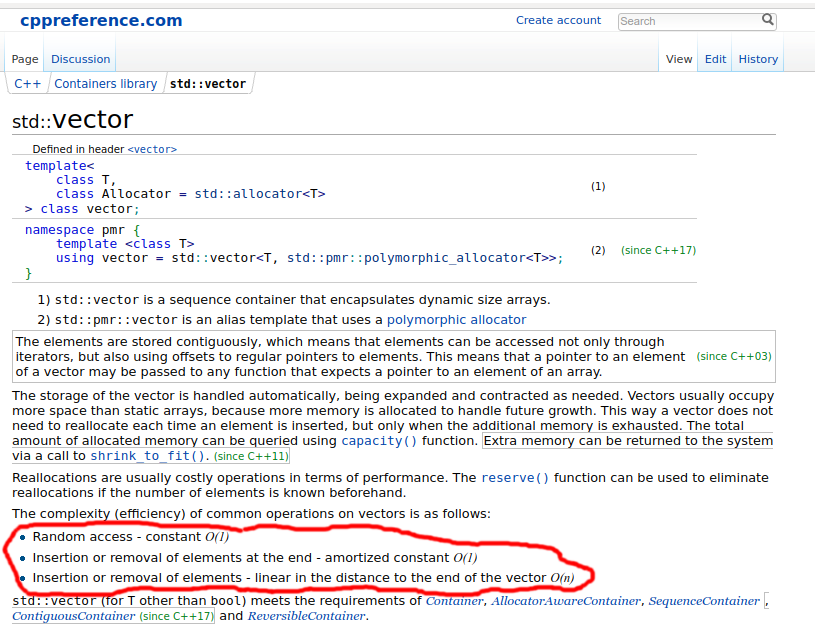
\includegraphics[width=8cm]{vector.png}
\end{frame}

\begin{frame}
    \frametitle{Vector -- time complexity}
    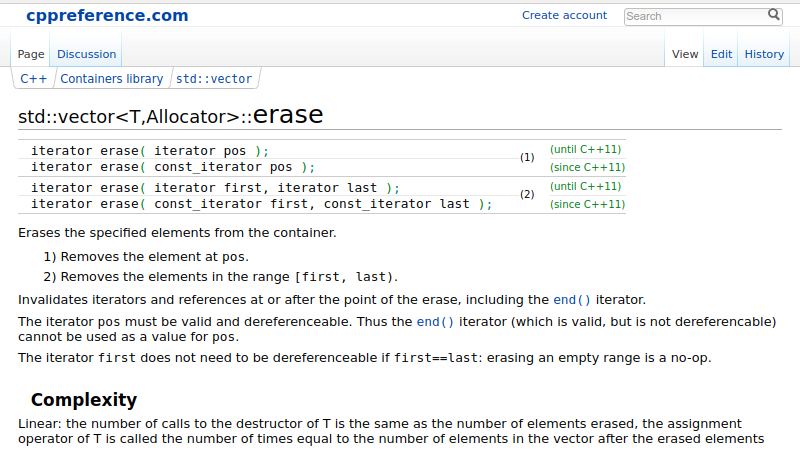
\includegraphics[width=11cm]{vector_erase.png}
\end{frame}

\begin{frame}
    \frametitle{Vector -- internal implementation}
    \centering
    \begin{tikzpicture}[ampersand replacement=\&]
\matrix (m) [matrix of nodes,
             nodes={draw, minimum size=8mm,anchor=center},
             nodes in empty cells, minimum height = 1cm,
             row 1/.style={nodes={draw=none}}]
{
  \node[draw=none, visible on=<1-6>] {0};
  \node[draw=none, visible on=<10->] {0};
  \&
  \node[draw=none, visible on=<1-6>] {1};
  \node[draw=none, visible on=<10->] {1};
  \&
  \node[draw=none, visible on=<10->] {2};
  \&
  \node[draw=none, visible on=<10->] {3};
  \&
  \node[draw=none, visible on=<10->] {4};
  \&
  \node[draw=none, visible on=<10->] {5};
  \&
  \node[draw=none, visible on=<10->] {6};
  \&
  \node[draw=none, visible on=<10->] {7};
  \\
  \node[draw, visible on=<1>] {};
  \node[draw, visible on=<2-6>] {4};
  \node[draw, visible on=<10>] {};
  \node[draw, visible on=<11->] {4};
  \&
  \node[draw, visible on=<1-2>] {};
  \node[draw, visible on=<3-6>] {12};
  \node[draw, visible on=<10-11>] {};
  \node[draw, visible on=<12->] {12};
  \&
  \node[draw, visible on=<10-12>] {};
  \node[draw, visible on=<13->] {1};
  \&
  \node[draw, visible on=<10-13>] {};
  \node[draw, visible on=<14->] {5};
  \&
  \node[draw, visible on=<10-15>] {};
  \node[draw, visible on=<16->] {87};
  \&
  \node[draw, visible on=<10->] {};
  \&
  \node[draw, visible on=<10->] {};
  \&
  \node[draw, visible on=<10->] {};
  \\
};
\begin{scope}[yshift=-2cm,xshift=-1.6cm]
\matrix (m) [matrix of nodes,
             nodes={draw, minimum size=8mm,anchor=center},
             nodes in empty cells, minimum height = 1cm,
             row 1/.style={nodes={draw=none}}]
{
  \node[draw=none, visible on=<4-14>] {0};
  \&
  \node[draw=none, visible on=<4-14>] {1};
  \&
  \node[draw=none, visible on=<4-14>] {2};
  \&
  \node[draw=none, visible on=<4-14>] {3};
  \\
  \node[draw, visible on=<4>] {};
  \node[draw, visible on=<5-14>] {4};
  \&
  \node[draw, visible on=<4-5>] {};
  \node[draw, visible on=<6-14>] {12};
  \&
  \node[draw, visible on=<4-7>] {};
  \node[draw, visible on=<8-14>] {1};
  \&
  \node[draw, visible on=<4-8>] {};
  \node[draw, visible on=<9-14>] {5};
  \\
};
\end{scope}
\end{tikzpicture}
\end{frame}

\begin{frame}
    \frametitle{Vector -- time complexity}
    \begin{itemize}
        \item \textit{insert (back)} \pause -- $O(1)$ (expected), \pause
        \item \textit{delete (back)} \pause -- $O(1)$, \pause
        \item \textit{lookup (index)} \pause -- $O(1)$, \pause
        \item \textit{insert (middle)} -- $O(N)$,
        \item \textit{delete (middle)} -- $O(N)$,
        \item \textit{find (value)} -- $O(N)$.
    \end{itemize}

    \pause
    \textcolor{gray}{
        Note: vector does not shrink by itself.
    }
\end{frame}

\begin{frame}
    \frametitle{Insert complexity proof.}
    Proof!
\end{frame}

\section{Balanced trees}

\subsection{BST}

\begin{frame}
    \frametitle{Binary search tree}
    Long long ago, before \texttt{c++11} \dots \pause all sets were based
    on the binary search trees.

    \centering
    \begin{tikzpicture}[>=stealth, every node/.style={circle, draw, minimum size=0.75cm}]
        \node (5) at (0,0) {$5$};
        \node (2) at (-2,-1.5) {$2$};
        \node (7) at (2,-1.5) {$7$};
        \node (1) at (-3,-3) {$1$};
        \node (3) at (-1,-3) {$3$};
        \node (15) at (3,-3) {$15$};
        \draw[->,draw] (5) -- (2);
        \draw[->,draw] (5) -- (7);
        \draw[->,draw] (2) -- (1);
        \draw[->,draw] (2) -- (3);
        \draw[->,draw] (7) -- (15);
    \end{tikzpicture}
\end{frame}

\subsection{AVL}

\begin{frame}
    \frametitle{AVL vs. BST}
    AVL is just a regular BST with rotations that guarantee reasonable
    time complexities. \pause

    \centering
    \includemovie{5cm}{5cm}{avl.gif}
\end{frame}

\begin{frame}
    \frametitle{AVL vs. BST -- worst case time complexity}
    \begin{columns}
    \begin{column}{0.5\textwidth}
    \centering
    \begin{block}{BST}
    \begin{itemize}
        \item \textit{insert} -- $O(N)$,
        \item \textit{delete} -- $O(N)$,
        \item \textit{lookup} -- $O(N)$.
    \end{itemize}
    \end{block}
    \end{column}
    \pause
    \begin{column}{0.5\textwidth}
    \centering
    \begin{block}{AVL}
    \begin{itemize}
        \item \textit{insert} -- $O(\log N)$,
        \item \textit{delete} -- $O(\log N)$,
        \item \textit{lookup} -- $O(\log N)$.
    \end{itemize}
    \end{block}
    \end{column}
    \end{columns}

    \pause
    \begin{block}{Note}
        \texttt{std::set} and \texttt{std::map} are internally using
        Red-Black Trees which have the same time complexity as AVL, but different
        internal constraints to ensure balancing.
    \end{block}
\end{frame}

\section{Hash tables}

\subsection{Idea}

\begin{frame}
    \frametitle{Hashing -- why do we need it?}

    \pause
    \begin{block}{}
    $U$ -- universe of numbers that may appear in the data.
    \end{block}

    What if $|U|$ is small (i.e. $1\,000\,000$)? \pause

    \medskip
    What if $|U|$ is large (i.e. $10^{18}$)? \pause

    \medskip
    ...then we need \textit{hashing}!
\end{frame}

\begin{frame}
    \frametitle{Hashing -- why do we need it?}
    \begin{block}{}
    $U$ -- universe of numbers that may appear in the data. \\
    $A$ -- array that we actually have. \\
    $M$ -- size of the array $A$.
    \end{block}

    \pause
    If we had a (fast) function $h : U \rightarrow \{0, \dots, M-1\}$, then we
    could store each element $x$ within $A[f(x)]$.

    \pause
    \textcolor{lightgray}{
    \textit{Note:} If $|U|$ is small, then the identity function $f(x) = x$
    would do.}

    \pause
    What could possibly go wrong? \pause
    \begin{itemize}
        \item what if we have a \textit{collision} ($f(x) = f(y)$)? \pause
        \item what if $f$ does \textbf{not} distribute elements uniformly over
            the available cells?
    \end{itemize}

\end{frame}

\subsection{Properties and limitations}

\begin{frame}
    \frametitle{Hashing -- properties}
    \begin{itemize}
        \item $f$ is an arithmetic expression,
            i.e. $f(x) = (5 \cdot x)\ \mathrm{mod}\ M$, \pause
        \item $f$ is randomly chosen from some set of functions
            (family), \pause
        \item \textit{collision} -- we store all the key-value pairs within
            a linked list, \pause
        \item a good family of functions ensures the correct distrubution
            (in expectation), \pause
        \item if the array gets full then all elements are rehashed into
            a bigger one. \pause
    \end{itemize}

    What are the time complexities of the operations?
    \begin{itemize}
        \item \textit{insert (no lookup)} -- \pause $O(1)$, \pause
        \item \textit{delete} -- \pause $O(1)$ (expected), \pause
        \item \textit{lookup} -- \pause $O(1)$ (expected).
    \end{itemize}
\end{frame}

\begin{frame}[fragile]
    \frametitle{Other data types}

    If a more complex data type needs to be stored, then it is necessary
    to define an own hash function and an equality operator. \pause What is more,
    \texttt{std::pair} is such a type, so STL does not provide any hash function
    for us (only the equality operator). \pause

    Example hash function for \texttt{std::pair<T1,T2>}:
    \begin{Verbatim}[commandchars=\\\{\},fontsize=\small]
struct pair_hash
\{
    template <class T1, class T2>
    std::size_t operator()
        (const std::pair<T1, T2> &pair) const
    \{
        return std::hash<T1>()(pair.first)
               ^ std::hash<T2>()(pair.second);
    \}
\};
\end{Verbatim}
\end{frame}

\begin{frame}[fragile]
    \frametitle{Other data types}

    If a more complex data type needs to be stored, then it is necessary
    to define an own hash function and an equality operator. What is more,
    \texttt{std::pair} is such a type, so STL does not provide any hash function
    for us (only the equality operator).

    Example hash function for \texttt{std::pair<T1,T2>}:
    \begin{Verbatim}[commandchars=\\\{\},fontsize=\small]
struct pair_hash
\{
    template <class T1, class T2>
    std::size_t operator()
        (const std::pair<T1, T2> &pair) const
    \{
        return \textcolor{red}{std::hash<T1>()(pair.first)}
               \textcolor{red}{^ std::hash<T2>()(pair.second);}
    \}
\};
\end{Verbatim}
\end{frame}

\begin{frame}[fragile]
    \frametitle{Other data types}

    If a more complex data type needs to be stored, then it is necessary
    to define an own hash function and an equality operator. What is more,
    \texttt{std::pair} is such a type, so STL does not provide any hash function
    for us (only the equality operator).

    Example hash function for \texttt{std::pair<T1,T2>}:
    \begin{Verbatim}[commandchars=\\\{\},fontsize=\small]
struct pair_hash
\{
    template <class T1, class T2>
    std::size_t operator()
        (const std::pair<T1, T2> &pair) const
    \{
        return std::hash<T1>()(pair.first)
               ^ (std::hash<T2>()(pair.second) << 1);
    \}
\};
\end{Verbatim}
\end{frame}

\begin{frame}
    \frametitle{Hashing -- limitations}
    \pause
    \begin{itemize}
        \item for small sets it's extremely inefficient due to rehashing, \pause
        \item for stored $N$ elements likely there will be a list
            of size $\Omega(\log \log N)$, \pause
        \item hashing function needs to be defined for the stored object
            (alternatively \texttt{operator<} in tree-based map), \pause
        \item for known hash function it is possible to prepare the data
            that will all fall into one place (linked list) causing
            the $\Omega(N)$ blow-up per single operation. \pause
    \end{itemize}

    \textcolor{gray}{\href{https://github.com/gcc-mirror/gcc/blob/5bea0e90e58d971cf3e67f784a116d81a20b927a/libstdc\%2B\%2B-v3/src/shared/hashtable-aux.cc}
        {\underline{Code!}}} \pause

    \begin{center}
    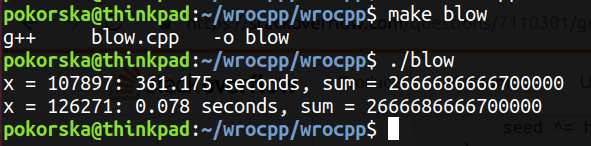
\includegraphics[width=9cm]{blow.png}
    \end{center}
\end{frame}

\begin{frame}
    \frametitle{Set vs. unordered set in practice}

    \textcolor{gray}{\underline{Code!}} \pause

    \centering
    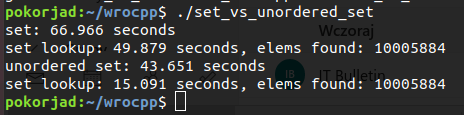
\includegraphics[width=8cm]{set_vs_uset.png}
\end{frame}

\subsection{Workarounds}

\begin{frame}
    \frametitle{Open addressing}
    Hash function: $hash(x) = x\ \mathrm{mod}\ 7$.

    \centering
    \begin{tikzpicture}[ampersand replacement=\&]
\matrix (m) [matrix of nodes,
             nodes={draw, minimum size=8mm,anchor=center},
             nodes in empty cells, minimum height = 1cm,
             row 1/.style={nodes={draw=none}},]
{
  0 \& 1 \& 2 \& 3 \& 4 \& 5 \& 6  \\
  \node[draw, visible on=<1-5>] {};
  \node[draw, visible on=<6>] {\textcolor{green}{84}};
  \node[draw, visible on=<7->] {84};
    \&   \&   \&
    \node[draw, visible on=<1-2>]{}; \node[draw, visible on=<3>]{\textcolor{green}{45}}; \node[draw, visible on=<4-8>]{45};
    \node[draw, visible on=<9>]{\textcolor{red}{45}}; \node[draw, visible on=<10-12>]{45};
    \node[draw, visible on=<13>]{\textcolor{red}{45}}; \node[draw, visible on=<14->]{45};
    \&
    \node[draw, visible on=<1-9>] {};
    \node[draw, visible on=<10>]{\textcolor{green}{17}}; \node[draw, visible on=<11->]{17};
    \node[draw, visible on=<14>]{\textcolor{red}{17}}; \node[draw, visible on=<15->]{17};
    \&
    \node[draw, visible on=<1-14>] {};
    \node[draw, visible on=<15>]{\textcolor{green}{3}}; \node[draw, visible on=<16->]{3};
    \&    \\
};

    \node[draw, circle, visible on=<2-3>] at (0,-2) {45};
    \node[draw, circle, visible on=<5-6>] at (0,-2) {84};
    \node[draw, circle, visible on=<8-10>] at (0,-2) {17};
    \node[draw, circle, visible on=<12-15>] at (0,-2) {3};

\end{tikzpicture}
\end{frame}

\begin{frame}
    \frametitle{Cuckoo-hashing (optional)}
    Idea of how to make the lookup in $O(1)$ in worst case (not expected).
\end{frame}

\begin{frame}
    \frametitle{The end}
    \centering
    Thank you.
\end{frame}

\end{document}
